% Options for packages loaded elsewhere
\PassOptionsToPackage{unicode}{hyperref}
\PassOptionsToPackage{hyphens}{url}
\PassOptionsToPackage{dvipsnames,svgnames,x11names}{xcolor}
%
\documentclass[
  11pt,
  a4paper,
  twoside,
  onecolumn]{article}
\title{Internet Appendix for Return Anomalies, Disagreement and Trading
Volume}
\author{Nikhil Vidhani}
\date{May 29, 2022}

\usepackage{amsmath,amssymb}
\usepackage{lmodern}
\usepackage{iftex}
\ifPDFTeX
  \usepackage[T1]{fontenc}
  \usepackage[utf8]{inputenc}
  \usepackage{textcomp} % provide euro and other symbols
\else % if luatex or xetex
  \usepackage{unicode-math}
  \defaultfontfeatures{Scale=MatchLowercase}
  \defaultfontfeatures[\rmfamily]{Ligatures=TeX,Scale=1}
\fi
% Use upquote if available, for straight quotes in verbatim environments
\IfFileExists{upquote.sty}{\usepackage{upquote}}{}
\IfFileExists{microtype.sty}{% use microtype if available
  \usepackage[]{microtype}
  \UseMicrotypeSet[protrusion]{basicmath} % disable protrusion for tt fonts
}{}
\usepackage{xcolor}
\IfFileExists{xurl.sty}{\usepackage{xurl}}{} % add URL line breaks if available
\IfFileExists{bookmark.sty}{\usepackage{bookmark}}{\usepackage{hyperref}}
\hypersetup{
  pdftitle={Internet Appendix for Return Anomalies, Disagreement and Trading Volume},
  pdfauthor={Nikhil Vidhani},
  colorlinks=true,
  linkcolor={red},
  filecolor={Maroon},
  citecolor={blue},
  urlcolor={blue},
  pdfcreator={LaTeX via pandoc}}
\urlstyle{same} % disable monospaced font for URLs
\usepackage[top=1.0in,bottom=1.0in,right=1.0in,left=1.0in]{geometry}
\usepackage{graphicx}
\makeatletter
\def\maxwidth{\ifdim\Gin@nat@width>\linewidth\linewidth\else\Gin@nat@width\fi}
\def\maxheight{\ifdim\Gin@nat@height>\textheight\textheight\else\Gin@nat@height\fi}
\makeatother
% Scale images if necessary, so that they will not overflow the page
% margins by default, and it is still possible to overwrite the defaults
% using explicit options in \includegraphics[width, height, ...]{}
\setkeys{Gin}{width=\maxwidth,height=\maxheight,keepaspectratio}
% Set default figure placement to htbp
\makeatletter
\def\fps@figure{htbp}
\makeatother
\setlength{\emergencystretch}{3em} % prevent overfull lines
\providecommand{\tightlist}{%
  \setlength{\itemsep}{0pt}\setlength{\parskip}{0pt}}
\setcounter{secnumdepth}{5}
\usepackage{letltxmacro}

\LetLtxMacro\Oldfootnote\footnote

\newcommand{\EnableFootNotes}{%
  \LetLtxMacro\footnote\Oldfootnote%
}

\newcommand{\DisableFootNotes}{%
  \renewcommand{\footnote}[2][]{\relax}
}
\usepackage[T1]{fontenc}
\usepackage[utf8]{inputenc}
\usepackage{booktabs}
\usepackage{longtable}
\usepackage{array}
\usepackage{multirow}
\usepackage{wrapfig}
\usepackage{float}
\usepackage{colortbl}
\usepackage{setspace}
\usepackage{pdflscape}
\usepackage{tabu}
\usepackage{threeparttable}
\usepackage{threeparttablex}
\usepackage[normalem]{ulem}
\usepackage{makecell}
\usepackage{xcolor}
\usepackage{rotating}
\usepackage{mathtools}
\usepackage{commath}
\usepackage[all]{hypcap}
\usepackage{placeins}
\usepackage{microtype}
\usepackage{tcolorbox}
\usepackage{pagecolor}
\usepackage{titling}
\setlength{\droptitle}{-10em}
\usepackage{amsmath}
\usepackage{siunitx}
\usepackage{xltabular}
\usepackage[font=normalfont]{subcaption}
\usepackage[skip=1ex, font=bf]{caption}
\setlength{\abovetopsep}{0.5ex}
\setlength{\belowrulesep}{0.5ex}
\usepackage{textcomp}
\usepackage{chngcntr}
\usepackage{ltablex}
\usepackage{comment}
\EnableFootNotes
\onehalfspacing
\usepackage{footmisc}
\setlength{\footnotemargin}{\parindent}
\renewcommand{\footnotelayout}{\setstretch{1}}
\setlength{\footnotesep}{\baselineskip}
\renewcommand{\footnotesize}{\small}
\usepackage{fancyhdr}
\pagestyle{fancy}
\fancyhf{}
\fancyhead[LE]{Nikhil Vidhani}
\fancyhead[RE]{Internet Appendix}
\fancyhead[CO]{Return Anomalies, Disagreement and Trading Volume}
\fancyfoot[C]{\thepage}
\usepackage[natbibapa]{apacite}
\bibliographystyle{apacite}
\ifLuaTeX
  \usepackage{selnolig}  % disable illegal ligatures
\fi

\begin{document}
\maketitle

% I need the below command to appear after natbib package in thesis_paper.tex file. This accomplishes that! I can't do that by including the below in preamble.tex
\renewcommand\bibsection{}
%\renewcommand\bibsection{\section*{\refname}}

\sisetup{input-open-uncertainty= ,  % <-- new
         input-close-uncertainty= , % <-- new
         table-space-text-pre=(,    % <-- new
         table-space-text-post=),   % <-- new
         table-align-text-pre=false,% <-- new
         table-format=1.3}

\defcitealias{kandel_pearson1995}{KP}
\defcitealias{chordia_etal2006}{CHS}

\renewcommand{\thesection}{IA.\arabic{section}}
\renewcommand{\thesubsection}{IA.\arabic{section}.\arabic{subsection}}
\renewcommand{\thesubsubsection}{IA.\arabic{section}.\arabic{subsection}.\arabic{subsubsection}}

\setcounter{page}{1}
\setcounter{figure}{0}
\setcounter{table}{0}
\setcounter{equation}{0}

\renewcommand{\thepage}{IA\textendash\arabic{page}}
\renewcommand\thefigure{IA.\arabic{figure}}    
\renewcommand\thetable{IA.\arabic{table}}    
\renewcommand\theequation{IA.\arabic{equation}}

\hypertarget{definition-of-anomalies}{%
\section{Definition of Anomalies}\label{definition-of-anomalies}}

Table \ref{tab:anomaly_list_extended} gives the list of thirty-nine
anomalies. Except for the momentum category, which are from
\cite{mclean_pontiff2016}, all other anomalies are from
\cite{roberts2018}. I also mention the original study and its findings,
construction using CRSP/COMPUSTAT variables.

\begin{landscape}\begingroup\fontsize{10}{12}\selectfont

\begin{spacing}{1.0}
\begin{longtable}[t]{>{\raggedleft\arraybackslash}p{1.8cm}>{\raggedright\arraybackslash}p{3.6cm}>{\raggedright\arraybackslash}p{3.6cm}>{\raggedright\arraybackslash}p{2.7cm}>{\raggedright\arraybackslash}p{2.7cm}>{\raggedright\arraybackslash}p{4.5cm}}
\caption{\label{tab:anomaly_list_extended}Anomalies List}\\
\multicolumn{6}{p{\linewidth}}{List of 39 anomalies used to construct the disagreement measure. Thirty-four anomalies are from \cite{roberts2018} and five momentum anomalies from \cite{mclean_pontiff2016}. The predicted relationship and the main table of findings is from the original study. Sixth column gives anomaly construction using CRSP/COMPUSTAT variables. Unless stated otherwise, $t$ captures time in years.}\\
\toprule
\textbf{Category / S.No.} & \textbf{Anomaly} & \textbf{Source} & \textbf{Predicted Relationship} & \textbf{Main Table} & \textbf{Construction}\\
\midrule
\endfirsthead
\caption[]{Anomalies List \textit{(continued)}}\\
\toprule
\textbf{Category / S.No.} & \textbf{Anomaly} & \textbf{Source} & \textbf{Predicted Relationship} & \textbf{Main Table} & \textbf{Construction}\\
\midrule
\endhead

\endfoot
\bottomrule
\endlastfoot
\addlinespace[0.3em]
\multicolumn{6}{l}{\textbf{Profitability}}\\
\hspace{1em}1 & Gross Profitability & \cite*{novymarx2013} & Positive & Table 1 & $GrProf = \left( revt_t - cogs_t \right) / at_t$\\
\hspace{1em}2 & Operating Profitability & \cite*{fama_french2015} & Positive & Table 1 Panel B & $OpProf = \left( revt_t - cogs_t - xint_t - xsga_t \right) / BE_t$\\
\hspace{1em}3 & Return on Assets & \cite*{haugen1996} & Positive & Table 3 & $RoA = ib_t / at_t$\\
\hspace{1em}4 & Return on Equity & \cite*{haugen1996} & Positive & Table 3 & $RoE = ib_t / BE_t$\\
\hspace{1em}5 & Profit Margin & \cite*{soliman2008} & Positive & Table 4 & $PfMg = oiadp_t / revt_t$\\
\hspace{1em}6 & Change in Asset Turnover & \cite*{soliman2008} & Positive & Table 4 & $ChgAssTurn = \Delta \left( revt_t / at_t \right)$\\
\addlinespace[0.3em]
\multicolumn{6}{l}{\textbf{Earnings Quality}}\\
\hspace{1em}7 & Accruals & \cite*{sloan1996} & Negative & Table 6 and 7 & $Accr = \frac{(\Delta act_t - \Delta che_t) - (\Delta lct_t - \Delta dlc_t - \Delta txp_t) - dp_t}{at_t}$\\
\hspace{1em}8 & Net Operating Assets & \cite*{hirshleifer_etal2004} & Negative & Table 5 & $NOA = \frac{(at_t - che_t ) - (at_t - dlc_t - dltt_t - BE_t)}{at_{t-1}}$\\
\hspace{1em}9 & Changes in Net Working Capital & \cite*{soliman2008} & Negative & Table 7 & $ChgNWC = \frac{\Delta (act_t - che_t) - \Delta (lct_t - dlc_t)}{at_t}$\\
\addlinespace[0.3em]
\multicolumn{6}{l}{\textbf{Valuation}}\\
\hspace{1em}10 & Book to market & \cite*{fama_french1992} & Positive & Table 6 & $BTM = BE_t / ME_t$\\
\hspace{1em}11 & Cash flow to price & \cite*{lakonishok_etal1994} & Positive & Table 4 & $CFP = \left( ib_t+dp_t \right) / ME_t$\\
\hspace{1em}12 & Earnings to Price & \cite*{basu1977} & Positive & Table 4 & $EP_t = ib_t / ME_t$\\
\hspace{1em}13 & Enterprise Multiple & \cite*{loughran_wellman2011} & Negative & Table 2 & $EntMult = \left( ME_t + dlc_t + dltt_t + pstkrv_t - che_t \right) / oibdp_t$\\
\hspace{1em}14 & Sales to price & \cite*{barbee_etal1996} & Positive & Table 2 & $SP = revt_t / ME_t$\\
\addlinespace[0.3em]
\multicolumn{6}{l}{\textbf{Momentum}}\\
\hspace{1em}15 & Short term momentum & \cite*{jegadeesh_titman1993} & Positive & Table 7 & $ret.6t2$, where $t$ is the current month\\
\hspace{1em}16 & Lagged Momentum & \cite*{novymarx2012} & Positive & Table 1 & $ret.12t7$, where $t$ is the current month\\
\hspace{1em}17 & Short-term reversal & \cite*{jegadeesh_titman1993} & Negative & Table 7 & $ret.1t1$, where $t$ is the current month\\
\hspace{1em}18 & Medium-term reversal & \cite*{jegadeesh_titman1993} & Negative & Table 7 & $ret.18t13$, where $t$ is the current month\\
\hspace{1em}19 & Long-term reversal & \cite*{debondt_thaler1985} & Negative &  & $ret.60t13$, where $t$ is the current month\\
\addlinespace[0.3em]
\multicolumn{6}{l}{\textbf{Investment}}\\
\hspace{1em}20 & Asset Growth & \cite*{cooper_etal2008} & Negative & Table III & $AssGr = \Delta at_t / at_{t-1}$\\
\hspace{1em}21 & Inventory Growth & \cite*{thomas_zhang2002} & Negative & Table 1 & $ChgInvt = \Delta invt_t  /  \overline{at_t}$\\
\hspace{1em}22 & Sales Growth & \cite*{lakonishok_etal1994} & Negative & Table 4 & $SalesGr = 5r_t + 4r_{t-1} + 3r_{t-2} + 2r_{t-3} + r_{t-4}$, where $r_t$ is the sales rank in year $t$\\
\hspace{1em}23 & Sustainable Growth & \cite*{lockwood2010} & Negative & Table 6 & $SustGr = \Delta BE_t  /  BE_{t-1}$\\
\hspace{1em}24 & CAPX Growth & \cite*{abarbanell_bushee1998} & Negative & Table 2 Panel B & $CapxGr = \left( capx_t - \overline{capx_{t-1}} \right)  /  \overline{capx_{t-1}}$\\
\hspace{1em}25 & Growth in Sales minus growth in Inventory & \cite*{abarbanell_bushee1998} & Positive & Table 2 Panel B & $SalesGr\_InvtGr = \left( \frac{revt_t - \overline{rev_{t-1}}}{\overline{rev_{t-1}}} \right)  /  \left( \frac{invt_t - \overline{invt_{t-1}}}{\overline{invt_{t-1}}} \right)$\\
\hspace{1em}26 & Investment Growth & \cite*{xing2007} & Negative & Table 4 & $InvstGr = \Delta capx_t / capx_{t-1}$\\
\hspace{1em}27 & Abnormal CAPX & \cite*{titman_etal2004} & Negative & Table 6 & $AbCapInvst = \left( \frac{capx_t/revt_t}{\frac{1}{3} \cdot \sum_{s=t-3}^{s=t-1} capx_s/rev_s} \right)$\\
\hspace{1em}28 & Investment to Capital Ratio & \cite*{xing2007} & Negative & Table 4 & $IK = capx_t / ppent_{t-1}$\\
\hspace{1em}29 & Investment to Asset Ratio & \cite*{lyandres_etal2007} & Negative & Section 4 & $IA = \left( \Delta ppent_t + \Delta invt_t \right)  /  at_{t-1}$\\
\addlinespace[0.3em]
\multicolumn{6}{l}{\textbf{Financing}}\\
\hspace{1em}30 & Increase in Debt Issuance & \cite*{spiess1999} & Negative &  & $DebtIssueInd = \left( \Delta dlc_t + \Delta dltt_t \right) / at_t$\\
\hspace{1em}31 & Leverage & \cite*{bhandari1988} & Positive & Table 2 Panel A & $LEV = dltt_t / ME_t$\\
\hspace{1em}32 & One year Share Issuance & \cite*{pontiff_woodgate2008} & Negative & Table 3 & $ShIssue\_1 = \left( shrout_t\ \cdot\ cfacshr_t \right)  /  \left( shrout_{t-1}\ \cdot\ cfacshr_{t-1} \right)$\\
\hspace{1em}33 & Five year Share Issuance & \cite*{daniel_titman2006} & Negative & Table 3 & $ShIssue\_1 = \left( shrout_t\ \cdot\ cfacshr_t \right)  /  \left( shrout_{t-5}\ \cdot\ cfacshr_{t-5} \right)$\\
\hspace{1em}34 & External Financing – I & \cite*{bradshaw_etal2006} & Negative & Table 5 & $ExtFin = \frac{(ShIssue\_1_t - 1) \cdot ME_t + \Delta dlc_t + \Delta dltt_t - dvc_t}{at_t}$\\
\hspace{1em}35 & External Financing – II & \cite*{bradshaw_etal2006} & Negative & Table 5 & $ExtFin2 = \frac{sstk_t - prstkc_t + dltis_t - dltr_t + dlcch_t - dv_t}{at_t}$\\
\addlinespace[0.3em]
\multicolumn{6}{l}{\textbf{Distress}}\\
\hspace{1em}36 & O-Score & \cite*{dichev1998} & Negative & Table 4 & $O\_Score = -1.32 -0.407 \cdot \log(\frac{at_t}{cpiind_t}) + 6.03 \cdot \frac{lt_t}{at_t} - 1.43 \cdot \frac{act_t - lct_t}{at_t} + 0.076 \cdot \frac{lct_t}{act_t} - 1.72 \cdot 1_{lt_t - at_t > 0} -2.37 \cdot \frac{ib_t}{at_t} -1.83 \cdot \frac{oiadp_t}{lt_t} + 0.285 \cdot1_{ib_t < 0,\ ib_{t-1} < 0} -0.521 \cdot \frac{\Delta ib_t}{\lvert ib_t \rvert + \lvert ib_{t-1} \rvert}$\\
\hspace{1em}37 & Z-Score & \cite*{dichev1998} & Positive & Table 3 & $Z\_Score = 1.2 \cdot \frac{act_t - lct_t}{at_t} + 1.4 \cdot \frac{re_t}{at_t} + 3.3 \cdot \frac{ni_t + xint_t + txp_t}{at_t} + 0.6 \cdot \frac{ME_t}{lt_t} + 1.0 \cdot \frac{revt_t}{at_t}$\\
\hspace{1em}38 & Distress Risk & \cite*{campbell_etal_distress} & Negative & Table 6 & 12-month horizon regression from Table 6\\
\addlinespace[0.3em]
\multicolumn{6}{l}{\textbf{Miscellaneous}}\\
\hspace{1em}39 & Industry Concentration & \cite*{industry_conc} & Negative & Table 3 & three-year simple average of the Herfindahl index computed on three-digit SIC codes and sales\\*
\end{longtable}
\end{spacing}
\endgroup{}
\end{landscape}

\hypertarget{robustness-checks}{%
\section{Robustness Checks}\label{robustness-checks}}

In this section I report several robustness regressions to strengthen
the trading volume results reported in Section 6.2.

\hypertarget{regressions-with-size-included}{%
\subsection{Regressions with size
included}\label{regressions-with-size-included}}

Evidence from Panel B of Table 3 suggests that the largest correlations
occur between \(L\_PRC\), \(L\_ME\), and \(NUMEST\); hence I chose to
exclude size (\(L\_ME\)) from regressions. Table
\ref{tab:reg_diff_specs_with_size} below presents regressions
specifications by augmenting logarithm of market size to the base
specification from Table 4.

The inclusion of \(L\_ME\) has a minute impact on STD\_DEV coefficient
and \(R^2\) (columns 1 and 3). Most noticeably, the coefficients on
\(BTM\) and \(EVOL\) become insignificant. This could be explained by a
size being in the denominator of these variables, and its inclusion
takes away any mechanical correlation of these variables with turnover.
The coefficients of \(L\_PRC\) and \(NUMEST\) also decline
substantially, proving the multi-collinearity concern evident from
correlations. Interestingly, the exclusion of \(L\_PRC\) in columns 4
and 6 make FDISP insignificant while increasing the coefficient on
\(L\_ME\). The coefficient of disagreement also reduces slightly owing
to the price being in the denominator of several anomalies. The relative
stability of the disagreement coefficient strengthens the case of
anomaly-driven disagreement, causing trading volume. Additionally, the
instability of FDISP casts doubts on its applicability as a measure of
disagreement. The negative correlation between \(FDISP\) and \(L\_PRC\)
(Table 3 Panel B) may be driving the positive association with turnover.

\begin{table}

\caption[Regression: Including Firm Size]{\label{tab:reg_diff_specs_with_size}Monthly cross-sectional regression: Including Firm Size}
\centering
\fontsize{9}{11}\selectfont
\begin{tabular}[t]{>{\raggedright\arraybackslash}p{3.5cm}>{\raggedright\arraybackslash}p{1.5cm}>{\raggedright\arraybackslash}p{1.5cm}>{\raggedright\arraybackslash}p{1.5cm}>{\raggedright\arraybackslash}p{1.5cm}>{\raggedright\arraybackslash}p{1.5cm}>{\raggedright\arraybackslash}p{1.5cm}}
\multicolumn{7}{p{\linewidth}}{Log turnover regressed on different set of explanatory variables and size: $L\_TURN_{i,t} = \beta \cdot STD\_DEV_{i,t-1} + \theta \cdot L\_ME_{i,t-1} + \alpha \cdot CONTROLS_{i,t-1} + \gamma \cdot DUMMIES_{i,t-1} + \epsilon_{i,t}$. All independent variables are one-month lagged variables. Definitions of all the variables appear in Appendix A.2. All regression specifications have industry and year fixed effects. \% $R^2$ explained is the percent of unexplained variation explained by including disagreement in the regression. Standard errors are double clustered by firm and year-month. Statistical significance of 10\%, 5\%, and 1\% are indicated by *, **, and *** respectively.}\\
\toprule

\multicolumn{1}{c}{ } & \multicolumn{6}{c}{$L\_TURN_t$} \\
\cmidrule(l{3pt}r{3pt}){2-7}
 & \phantom{-}(1) & \phantom{-}(2) & \phantom{-}(3) & \phantom{-}(4) & \phantom{-}(5) & \phantom{-}(6)\\
\midrule
$STD\_DEV_{t-1}$ & $\phantom{-}1.575$*** &  & $\phantom{-}1.586$*** & $\phantom{-}1.421$*** & $\phantom{-}1.650$*** & $\phantom{-}1.503$***\\
 & (\phantom{-}$0.062$) &  & (\phantom{-}$0.061$) & (\phantom{-}$0.060$) & (\phantom{-}$0.062$) & (\phantom{-}$0.061$)\\
\addlinespace
$FDISP_{t-1}$ & $\phantom{-}0.010$ & $\phantom{-}0.030$*** & $\phantom{-}0.012$* & $-0.003$ & $\phantom{-}0.011$* & $-0.002$\\
 & (\phantom{-}$0.006$) & (\phantom{-}$0.006$) & (\phantom{-}$0.006$) & (\phantom{-}$0.006$) & (\phantom{-}$0.006$) & (\phantom{-}$0.006$)\\
\addlinespace
$L\_ME_{t-1}$ &  & $\phantom{-}0.103$*** & $\phantom{-}0.105$*** & $\phantom{-}0.169$*** & $\phantom{-}0.192$*** & $\phantom{-}0.235$***\\
 &  & (\phantom{-}$0.011$) & (\phantom{-}$0.011$) & (\phantom{-}$0.010$) & (\phantom{-}$0.008$) & (\phantom{-}$0.007$)\\
\addlinespace
$NASDAQ$ & $\phantom{-}0.125$*** & $\phantom{-}0.186$*** & $\phantom{-}0.168$*** & $\phantom{-}0.176$*** & $\phantom{-}0.182$*** & $\phantom{-}0.187$***\\
 & (\phantom{-}$0.022$) & (\phantom{-}$0.022$) & (\phantom{-}$0.021$) & (\phantom{-}$0.021$) & (\phantom{-}$0.022$) & (\phantom{-}$0.022$)\\
\addlinespace
$RET^+_{t-1}$ & $\phantom{-}1.554$*** & $\phantom{-}1.733$*** & $\phantom{-}1.551$*** & $\phantom{-}1.535$*** & $\phantom{-}1.528$*** & $\phantom{-}1.517$***\\
 & (\phantom{-}$0.062$) & (\phantom{-}$0.068$) & (\phantom{-}$0.062$) & (\phantom{-}$0.063$) & (\phantom{-}$0.061$) & (\phantom{-}$0.062$)\\
\addlinespace
$RET^-_{t-1}$ & $-2.232$*** & $-2.464$*** & $-2.231$*** & $-2.052$*** & $-2.277$*** & $-2.120$***\\
 & (\phantom{-}$0.075$) & (\phantom{-}$0.082$) & (\phantom{-}$0.076$) & (\phantom{-}$0.076$) & (\phantom{-}$0.076$) & (\phantom{-}$0.077$)\\
\addlinespace
$LEV_{t-1}$ & $\phantom{-}0.061$*** & $\phantom{-}0.072$*** & $\phantom{-}0.058$*** & $\phantom{-}0.054$*** & $\phantom{-}0.057$*** & $\phantom{-}0.053$***\\
 & (\phantom{-}$0.007$) & (\phantom{-}$0.007$) & (\phantom{-}$0.007$) & (\phantom{-}$0.007$) & (\phantom{-}$0.007$) & (\phantom{-}$0.007$)\\
\addlinespace
$CAPM\_\beta_{t-1}$ & $\phantom{-}0.089$*** & $\phantom{-}0.081$** & $\phantom{-}0.084$*** & $\phantom{-}0.084$*** & $\phantom{-}0.081$*** & $\phantom{-}0.081$***\\
 & (\phantom{-}$0.030$) & (\phantom{-}$0.032$) & (\phantom{-}$0.030$) & (\phantom{-}$0.030$) & (\phantom{-}$0.030$) & (\phantom{-}$0.030$)\\
\addlinespace
$BTM_{t-1}$ & $\phantom{-}0.022$* & $\phantom{-}0.023$* & $\phantom{-}0.045$*** & $\phantom{-}0.038$*** & $\phantom{-}0.063$*** & $\phantom{-}0.055$***\\
 & (\phantom{-}$0.012$) & (\phantom{-}$0.012$) & (\phantom{-}$0.012$) & (\phantom{-}$0.012$) & (\phantom{-}$0.012$) & (\phantom{-}$0.012$)\\
\addlinespace
$L\_PRC_{t-1}$ & $\phantom{-}0.231$*** & $\phantom{-}0.113$*** & $\phantom{-}0.150$*** &  & $\phantom{-}0.123$*** & \\
 & (\phantom{-}$0.012$) & (\phantom{-}$0.013$) & (\phantom{-}$0.013$) &  & (\phantom{-}$0.013$) & \\
\addlinespace
$L\_FAGE_{t-1}$ & $-0.128$*** & $-0.174$*** & $-0.149$*** & $-0.150$*** & $-0.152$*** & $-0.153$***\\
 & (\phantom{-}$0.012$) & (\phantom{-}$0.013$) & (\phantom{-}$0.013$) & (\phantom{-}$0.013$) & (\phantom{-}$0.013$) & (\phantom{-}$0.013$)\\
\addlinespace
$ESURP_{t-1}$ & $\phantom{-}0.248$*** & $\phantom{-}0.277$*** & $\phantom{-}0.234$*** & $\phantom{-}0.197$*** & $\phantom{-}0.236$*** & $\phantom{-}0.204$***\\
 & (\phantom{-}$0.031$) & (\phantom{-}$0.035$) & (\phantom{-}$0.032$) & (\phantom{-}$0.032$) & (\phantom{-}$0.033$) & (\phantom{-}$0.032$)\\
\addlinespace
$EVOL_{t-1}$ & $\phantom{-}0.001$ & $\phantom{-}0.126$*** & $\phantom{-}0.004$ & $-0.098$** & $\phantom{-}0.012$ & $-0.075$\\
 & (\phantom{-}$0.044$) & (\phantom{-}$0.045$) & (\phantom{-}$0.044$) & (\phantom{-}$0.047$) & (\phantom{-}$0.044$) & (\phantom{-}$0.047$)\\
\addlinespace
$NUMEST_{t-1}$ & $\phantom{-}0.034$*** & $\phantom{-}0.023$*** & $\phantom{-}0.021$*** & $\phantom{-}0.018$*** &  & \\
 & (\phantom{-}$0.001$) & (\phantom{-}$0.002$) & (\phantom{-}$0.002$) & (\phantom{-}$0.002$) &  & \\
 &  &  &  &  &  \vphantom{1} & \\
\midrule
 &  &  &  &  &  & \\
$\textrm{Adj.} \: R^2$ & {$\phantom{-}0.406$} & {$\phantom{-}0.396$} & {$\phantom{-}0.412$} & {$\phantom{-}0.406$} & {$\phantom{-}0.404$} & {$\phantom{-}0.399$}\\
$\% \: R^2 \: \textrm{Explained}$ & {$\phantom{-}4.550$} & {} & {$\phantom{-}4.960$} & {$\phantom{-}4.170$} & {$\phantom{-}5.500$} & {$\phantom{-}4.690$}\\
$\textrm{Observations}$ & {\phantom{-}954,029} & {\phantom{-}954,029} & {\phantom{-}954,029} & {\phantom{-}954,029} & {\phantom{-}954,029} & {\phantom{-}954,029}\\
\bottomrule
\end{tabular}
\end{table}

\hypertarget{financial-firms}{%
\subsection{Financial Firms}\label{financial-firms}}

Table \ref{tab:reg_fin_and_nonfin_firms} shows regression results for
all firms, financial firms ,and non-financial firms. Results indicate
that the disagreement-volume relationship is significant both
statistically and economically, irrespective of whether financial firms
are included in the sample. Interestingly, in the smaller sample of just
financial firms (columns 3 and 4), the coefficients on \(NASDAQ\),
\(LEV\), \(BTM\), \(FAGE\), and \(FDISP\) lose significance.

\begin{table}

\caption[Regression: Financial Firms]{\label{tab:reg_fin_and_nonfin_firms}Monthly cross-sectional regression: Financial Firms}
\centering
\fontsize{9}{11}\selectfont
\begin{tabular}[t]{>{\raggedright\arraybackslash}p{3.5cm}>{\raggedright\arraybackslash}p{1.5cm}>{\raggedright\arraybackslash}p{1.5cm}>{\raggedright\arraybackslash}p{1.5cm}>{\raggedright\arraybackslash}p{1.5cm}>{\raggedright\arraybackslash}p{1.5cm}>{\raggedright\arraybackslash}p{1.5cm}}
\multicolumn{7}{p{\linewidth}}{Log turnover regressed on different set of explanatory variables: $L\_TURN_{i,t} = \beta \cdot STD\_DEV_{i,t-1} + \alpha \cdot CONTROLS_{i,t-1} + \gamma \cdot DUMMIES_{i,t-1} + \epsilon_{i,t}$ for financial and non-financial firms. Financial firms are identified with starting SIC code of $6$. All independent variables are one-month lagged variables. Definitions of all the variables appear in Appendix A.2. All regression specifications have industry and year fixed effects. \% $R^2$ explained is the percent of unexplained variation explained by including disagreement in the regression. Standard errors are double clustered by firm and year-month. Statistical significance of 10\%, 5\%, and 1\% are indicated by *, **, and *** respectively.}\\
\toprule

\multicolumn{1}{c}{ } & \multicolumn{6}{c}{$L\_TURN_t$} \\
\cmidrule(l{3pt}r{3pt}){2-7}
\multicolumn{1}{c}{ } & \multicolumn{2}{c}{All firms} & \multicolumn{2}{c}{Financial Firms} & \multicolumn{2}{c}{Non-financial Firms} \\
\cmidrule(l{3pt}r{3pt}){2-3} \cmidrule(l{3pt}r{3pt}){4-5} \cmidrule(l{3pt}r{3pt}){6-7}
 & \phantom{-}(1) & \phantom{-}(2) & \phantom{-}(3) & \phantom{-}(4) & \phantom{-}(5) & \phantom{-}(6)\\
\midrule
$STD\_DEV_{t-1}$ &  & $\phantom{-}1.575$*** &  & $\phantom{-}1.445$*** &  & $\phantom{-}1.551$***\\
 &  & (\phantom{-}$0.062$) &  & (\phantom{-}$0.161$) &  & (\phantom{-}$0.065$)\\
\addlinespace
$FDISP_{t-1}$ & $\phantom{-}0.029$*** & $\phantom{-}0.010$ & $\phantom{-}0.042$** & $\phantom{-}0.028$ & $\phantom{-}0.025$*** & $\phantom{-}0.007$\\
 & (\phantom{-}$0.006$) & (\phantom{-}$0.006$) & (\phantom{-}$0.019$) & (\phantom{-}$0.018$) & (\phantom{-}$0.007$) & (\phantom{-}$0.007$)\\
\addlinespace
$NASDAQ$ & $\phantom{-}0.143$*** & $\phantom{-}0.125$*** & $-0.041$ & $-0.032$ & $\phantom{-}0.195$*** & $\phantom{-}0.171$***\\
 & (\phantom{-}$0.022$) & (\phantom{-}$0.022$) & (\phantom{-}$0.043$) & (\phantom{-}$0.042$) & (\phantom{-}$0.024$) & (\phantom{-}$0.024$)\\
\addlinespace
$RET^+_{t-1}$ & $\phantom{-}1.735$*** & $\phantom{-}1.554$*** & $\phantom{-}2.013$*** & $\phantom{-}1.845$*** & $\phantom{-}1.661$*** & $\phantom{-}1.488$***\\
 & (\phantom{-}$0.068$) & (\phantom{-}$0.062$) & (\phantom{-}$0.109$) & (\phantom{-}$0.100$) & (\phantom{-}$0.067$) & (\phantom{-}$0.061$)\\
\addlinespace
$RET^-_{t-1}$ & $-2.463$*** & $-2.232$*** & $-2.940$*** & $-2.737$*** & $-2.372$*** & $-2.150$***\\
 & (\phantom{-}$0.082$) & (\phantom{-}$0.075$) & (\phantom{-}$0.162$) & (\phantom{-}$0.152$) & (\phantom{-}$0.079$) & (\phantom{-}$0.072$)\\
\addlinespace
$LEV_{t-1}$ & $\phantom{-}0.075$*** & $\phantom{-}0.061$*** & $\phantom{-}0.055$*** & $\phantom{-}0.046$*** & $\phantom{-}0.080$*** & $\phantom{-}0.066$***\\
 & (\phantom{-}$0.007$) & (\phantom{-}$0.007$) & (\phantom{-}$0.013$) & (\phantom{-}$0.013$) & (\phantom{-}$0.008$) & (\phantom{-}$0.008$)\\
\addlinespace
$CAPM\_\beta_{t-1}$ & $\phantom{-}0.086$*** & $\phantom{-}0.089$*** & $\phantom{-}0.140$*** & $\phantom{-}0.146$*** & $\phantom{-}0.078$** & $\phantom{-}0.082$***\\
 & (\phantom{-}$0.031$) & (\phantom{-}$0.030$) & (\phantom{-}$0.044$) & (\phantom{-}$0.044$) & (\phantom{-}$0.032$) & (\phantom{-}$0.030$)\\
\addlinespace
$BTM_{t-1}$ & $\phantom{-}0.001$ & $\phantom{-}0.022$* & $-0.020$ & $-0.014$ & $\phantom{-}0.001$ & $\phantom{-}0.022$*\\
 & (\phantom{-}$0.012$) & (\phantom{-}$0.012$) & (\phantom{-}$0.024$) & (\phantom{-}$0.023$) & (\phantom{-}$0.013$) & (\phantom{-}$0.013$)\\
\addlinespace
$L\_PRC_{t-1}$ & $\phantom{-}0.193$*** & $\phantom{-}0.231$*** & $\phantom{-}0.075$*** & $\phantom{-}0.106$*** & $\phantom{-}0.218$*** & $\phantom{-}0.257$***\\
 & (\phantom{-}$0.012$) & (\phantom{-}$0.012$) & (\phantom{-}$0.027$) & (\phantom{-}$0.028$) & (\phantom{-}$0.013$) & (\phantom{-}$0.013$)\\
\addlinespace
$L\_FAGE_{t-1}$ & $-0.153$*** & $-0.128$*** & $-0.061$* & $-0.054$* & $-0.158$*** & $-0.133$***\\
 & (\phantom{-}$0.013$) & (\phantom{-}$0.012$) & (\phantom{-}$0.032$) & (\phantom{-}$0.031$) & (\phantom{-}$0.014$) & (\phantom{-}$0.013$)\\
\addlinespace
$ESURP_{t-1}$ & $\phantom{-}0.290$*** & $\phantom{-}0.248$*** & $\phantom{-}0.210$*** & $\phantom{-}0.193$*** & $\phantom{-}0.310$*** & $\phantom{-}0.265$***\\
 & (\phantom{-}$0.035$) & (\phantom{-}$0.031$) & (\phantom{-}$0.061$) & (\phantom{-}$0.060$) & (\phantom{-}$0.036$) & (\phantom{-}$0.033$)\\
\addlinespace
$EVOL_{t-1}$ & $\phantom{-}0.122$*** & $\phantom{-}0.001$ & $\phantom{-}0.120$ & $\phantom{-}0.002$ & $\phantom{-}0.121$** & $\phantom{-}0.006$\\
 & (\phantom{-}$0.045$) & (\phantom{-}$0.044$) & (\phantom{-}$0.119$) & (\phantom{-}$0.117$) & (\phantom{-}$0.048$) & (\phantom{-}$0.047$)\\
\addlinespace
$NUMEST_{t-1}$ & $\phantom{-}0.035$*** & $\phantom{-}0.034$*** & $\phantom{-}0.049$*** & $\phantom{-}0.048$*** & $\phantom{-}0.032$*** & $\phantom{-}0.031$***\\
 & (\phantom{-}$0.001$) & (\phantom{-}$0.001$) & (\phantom{-}$0.003$) & (\phantom{-}$0.003$) & (\phantom{-}$0.002$) & (\phantom{-}$0.002$)\\
 &  &  &  &  &  \vphantom{1} & \\
\midrule
 &  &  &  &  &  & \\
$\textrm{Adj.} \: R^2$ & {$\phantom{-}0.391$} & {$\phantom{-}0.406$} & {$\phantom{-}0.351$} & {$\phantom{-}0.362$} & {$\phantom{-}0.388$} & {$\phantom{-}0.404$}\\
$\% \: R^2 \: \textrm{Explained}$ & {} & {$\phantom{-}4.550$} & {} & {$\phantom{-}3.770$} & {} & {$\phantom{-}4.580$}\\
$\textrm{Observations}$ & {\phantom{-}954,029} & {\phantom{-}954,029} & {\phantom{-}154,065} & {\phantom{-}154,065} & {\phantom{-}799,964} & {\phantom{-}799,964}\\
\bottomrule
\end{tabular}
\end{table}

\hypertarget{sp-500-membership}{%
\subsection{S\&P 500 Membership}\label{sp-500-membership}}

Evidence from Table \ref{tab:reg_sp500_membership} suggests that the
disagreement-volume relationship is stronger for non S\&P-500 firms.

\begin{table}

\caption[Regression: S\&P 500 Membership]{\label{tab:reg_sp500_membership}Monthly cross-sectional regression: S\&P 500 Membership}
\centering
\fontsize{9}{11}\selectfont
\begin{tabular}[t]{>{\raggedright\arraybackslash}p{2.6cm}>{\raggedright\arraybackslash}p{1.1cm}>{\raggedright\arraybackslash}p{1.1cm}>{\raggedright\arraybackslash}p{1.1cm}>{\raggedright\arraybackslash}p{1.1cm}>{\raggedright\arraybackslash}p{1.1cm}>{\raggedright\arraybackslash}p{1.1cm}>{\raggedright\arraybackslash}p{1.1cm}>{\raggedright\arraybackslash}p{1.1cm}}
\multicolumn{9}{p{\linewidth}}{Log turnover regressed on different set of explanatory variables and size: $L\_TURN_{i,t} = \beta \cdot STD\_DEV_{i,t-1} + \theta \cdot L\_ME_{i,t-1} + \alpha \cdot CONTROLS_{i,t-1} + \gamma \cdot DUMMIES_{i,t-1} + \epsilon_{i,t}$. Also included is a dummy for S\&P 500 membership. All independent variables are one-month lagged variables. Definitions of all the variables appear in Appendix A.2. All regression specifications have industry and year fixed effects. \% $R^2$ explained is the percent of unexplained variation explained by including disagreement in the regression. Standard errors are double clustered by firm and year-month. Statistical significance of 10\%, 5\%, and 1\% are indicated by *, **, and *** respectively.}\\
\toprule

\multicolumn{1}{c}{ } & \multicolumn{8}{c}{$L\_TURN_t$} \\
\cmidrule(l{3pt}r{3pt}){2-9}
\multicolumn{1}{c}{ } & \multicolumn{2}{c}{S\&P 500 firms} & \multicolumn{2}{c}{Non S\&P 500 firms} & \multicolumn{4}{c}{All firms} \\
\cmidrule(l{3pt}r{3pt}){2-3} \cmidrule(l{3pt}r{3pt}){4-5} \cmidrule(l{3pt}r{3pt}){6-9}
 & \phantom{-}(1) & \phantom{-}(2) & \phantom{-}(3) & \phantom{-}(4) & \phantom{-}(5) & \phantom{-}(6) & \phantom{-}(7) & \phantom{-}(8)\\
\midrule
$STD\_DEV_{t-1}$ &  & $\phantom{-}0.935$*** &  & $\phantom{-}1.641$*** &  & $\phantom{-}1.575$*** & $\phantom{-}1.574$*** & $\phantom{-}1.672$***\\
 &  & (\phantom{-}$0.098$) &  & (\phantom{-}$0.064$) &  & (\phantom{-}$0.062$) & (\phantom{-}$0.062$) & (\phantom{-}$0.068$)\\
\addlinespace
$FDISP_{t-1}$ & $\phantom{-}0.045$*** & $\phantom{-}0.028$** & $\phantom{-}0.032$*** & $\phantom{-}0.015$** & $\phantom{-}0.029$*** & $\phantom{-}0.010$ & $\phantom{-}0.011$* & $-0.005$\\
 & (\phantom{-}$0.012$) & (\phantom{-}$0.012$) & (\phantom{-}$0.006$) & (\phantom{-}$0.006$) & (\phantom{-}$0.006$) & (\phantom{-}$0.006$) & (\phantom{-}$0.006$) & (\phantom{-}$0.007$)\\
\addlinespace
$SP500$ &  &  &  &  &  &  & $-0.083$*** & $\phantom{-}0.238$**\\
 &  &  &  &  &  &  & (\phantom{-}$0.023$) & (\phantom{-}$0.106$)\\
\addlinespace
$STD\_DEV_{t-1} \times SP500$ &  &  &  &  &  &  &  & $-0.485$***\\
 &  &  &  &  &  &  &  & (\phantom{-}$0.149$)\\
\addlinespace
$FDISP_{t-1} \times SP500$ &  &  &  &  &  &  &  & $\phantom{-}0.166$***\\
 &  &  &  &  &  &  &  & (\phantom{-}$0.019$)\\
\addlinespace
$NASDAQ$ & $\phantom{-}0.279$*** & $\phantom{-}0.253$*** & $\phantom{-}0.169$*** & $\phantom{-}0.153$*** & $\phantom{-}0.143$*** & $\phantom{-}0.125$*** & $\phantom{-}0.121$*** & $\phantom{-}0.121$***\\
 & (\phantom{-}$0.040$) & (\phantom{-}$0.039$) & (\phantom{-}$0.023$) & (\phantom{-}$0.022$) & (\phantom{-}$0.022$) & (\phantom{-}$0.022$) & (\phantom{-}$0.022$) & (\phantom{-}$0.022$)\\
\addlinespace
$RET^+_{t-1}$ & $\phantom{-}1.533$*** & $\phantom{-}1.404$*** & $\phantom{-}1.703$*** & $\phantom{-}1.524$*** & $\phantom{-}1.735$*** & $\phantom{-}1.554$*** & $\phantom{-}1.549$*** & $\phantom{-}1.543$***\\
 & (\phantom{-}$0.078$) & (\phantom{-}$0.074$) & (\phantom{-}$0.067$) & (\phantom{-}$0.062$) & (\phantom{-}$0.068$) & (\phantom{-}$0.062$) & (\phantom{-}$0.062$) & (\phantom{-}$0.061$)\\
\addlinespace
$RET^-_{t-1}$ & $-1.989$*** & $-1.840$*** & $-2.389$*** & $-2.158$*** & $-2.463$*** & $-2.232$*** & $-2.226$*** & $-2.220$***\\
 & (\phantom{-}$0.144$) & (\phantom{-}$0.138$) & (\phantom{-}$0.075$) & (\phantom{-}$0.069$) & (\phantom{-}$0.082$) & (\phantom{-}$0.075$) & (\phantom{-}$0.075$) & (\phantom{-}$0.074$)\\
\addlinespace
$LEV_{t-1}$ & $\phantom{-}0.072$*** & $\phantom{-}0.058$*** & $\phantom{-}0.064$*** & $\phantom{-}0.052$*** & $\phantom{-}0.075$*** & $\phantom{-}0.061$*** & $\phantom{-}0.061$*** & $\phantom{-}0.061$***\\
 & (\phantom{-}$0.012$) & (\phantom{-}$0.011$) & (\phantom{-}$0.007$) & (\phantom{-}$0.007$) & (\phantom{-}$0.007$) & (\phantom{-}$0.007$) & (\phantom{-}$0.007$) & (\phantom{-}$0.007$)\\
\addlinespace
$CAPM\_\beta_{t-1}$ & $\phantom{-}0.044$ & $\phantom{-}0.040$ & $\phantom{-}0.086$*** & $\phantom{-}0.091$*** & $\phantom{-}0.086$*** & $\phantom{-}0.089$*** & $\phantom{-}0.089$*** & $\phantom{-}0.088$***\\
 & (\phantom{-}$0.044$) & (\phantom{-}$0.043$) & (\phantom{-}$0.032$) & (\phantom{-}$0.030$) & (\phantom{-}$0.031$) & (\phantom{-}$0.030$) & (\phantom{-}$0.030$) & (\phantom{-}$0.030$)\\
\addlinespace
$BTM_{t-1}$ & $\phantom{-}0.149$*** & $\phantom{-}0.159$*** & $-0.022$* & $\phantom{-}0.000$ & $\phantom{-}0.001$ & $\phantom{-}0.022$* & $\phantom{-}0.023$* & $\phantom{-}0.023$*\\
 & (\phantom{-}$0.018$) & (\phantom{-}$0.018$) & (\phantom{-}$0.012$) & (\phantom{-}$0.012$) & (\phantom{-}$0.012$) & (\phantom{-}$0.012$) & (\phantom{-}$0.012$) & \vphantom{1} (\phantom{-}$0.012$)\\
\addlinespace
$L\_PRC_{t-1}$ & $-0.026$ & $-0.020$ & $\phantom{-}0.194$*** & $\phantom{-}0.237$*** & $\phantom{-}0.193$*** & $\phantom{-}0.231$*** & $\phantom{-}0.233$*** & $\phantom{-}0.235$***\\
 & (\phantom{-}$0.018$) & (\phantom{-}$0.018$) & (\phantom{-}$0.012$) & (\phantom{-}$0.012$) & (\phantom{-}$0.012$) & (\phantom{-}$0.012$) & (\phantom{-}$0.012$) & (\phantom{-}$0.012$)\\
\addlinespace
$L\_FAGE_{t-1}$ & $-0.143$*** & $-0.127$*** & $-0.116$*** & $-0.092$*** & $-0.153$*** & $-0.128$*** & $-0.117$*** & $-0.118$***\\
 & (\phantom{-}$0.024$) & (\phantom{-}$0.023$) & (\phantom{-}$0.013$) & (\phantom{-}$0.013$) & (\phantom{-}$0.013$) & (\phantom{-}$0.012$) & (\phantom{-}$0.012$) & (\phantom{-}$0.012$)\\
\addlinespace
$ESURP_{t-1}$ & $\phantom{-}0.143$* & $\phantom{-}0.122$* & $\phantom{-}0.316$*** & $\phantom{-}0.272$*** & $\phantom{-}0.290$*** & $\phantom{-}0.248$*** & $\phantom{-}0.249$*** & $\phantom{-}0.245$***\\
 & (\phantom{-}$0.078$) & (\phantom{-}$0.071$) & (\phantom{-}$0.034$) & (\phantom{-}$0.031$) & (\phantom{-}$0.035$) & (\phantom{-}$0.031$) & (\phantom{-}$0.032$) & (\phantom{-}$0.032$)\\
\addlinespace
$EVOL_{t-1}$ & $\phantom{-}0.024$ & $-0.095$ & $\phantom{-}0.216$*** & $\phantom{-}0.093$** & $\phantom{-}0.122$*** & $\phantom{-}0.001$ & $\phantom{-}0.004$ & $\phantom{-}0.000$\\
 & (\phantom{-}$0.113$) & (\phantom{-}$0.105$) & (\phantom{-}$0.046$) & (\phantom{-}$0.044$) & (\phantom{-}$0.045$) & (\phantom{-}$0.044$) & (\phantom{-}$0.044$) & (\phantom{-}$0.044$)\\
\addlinespace
$NUMEST_{t-1}$ & $\phantom{-}0.005$*** & $\phantom{-}0.005$*** & $\phantom{-}0.064$*** & $\phantom{-}0.062$*** & $\phantom{-}0.035$*** & $\phantom{-}0.034$*** & $\phantom{-}0.036$*** & $\phantom{-}0.037$***\\
 & (\phantom{-}$0.002$) & (\phantom{-}$0.002$) & (\phantom{-}$0.002$) & (\phantom{-}$0.002$) & (\phantom{-}$0.001$) & (\phantom{-}$0.001$) & (\phantom{-}$0.002$) & (\phantom{-}$0.002$)\\
 &  &  &  &  &  &  &  \vphantom{1} & \\
\midrule
 &  &  &  &  &  &  &  & \\
$\textrm{Adj.} \: R^2$ & {$\phantom{-}0.628$} & {$\phantom{-}0.635$} & {$\phantom{-}0.404$} & {$\phantom{-}0.419$} & {$\phantom{-}0.391$} & {$\phantom{-}0.406$} & {$\phantom{-}0.407$} & {$\phantom{-}0.408$}\\
$\textrm{Observations}$ & {\phantom{-}202,257} & {\phantom{-}202,257} & {\phantom{-}751,772} & {\phantom{-}751,772} & {\phantom{-}954,029} & {\phantom{-}954,029} & {\phantom{-}954,029} & {\phantom{-}954,029}\\
\bottomrule
\end{tabular}
\end{table}

\hypertarget{book-to-market-splits}{%
\subsection{Book to market splits}\label{book-to-market-splits}}

Investment using accounting fundamentals and related ratios is popular
among value investors. Several books on value investing give prominence
to price to book ratio as an indicator of value firms\footnote{Lower P/B
  ratio (or high book to market) signifies that a firm's market price
  does not accurately reflect its book value and is undervalued.
  \cite{graham1965} is a popular investing book following value
  investing tenets.}. Value investment attempts to estimate the
intrinsic value of a stock using information from the balance sheet and
profit and loss statements. The intrinsic value is then compared to the
current stock price, and a buy (sell) trade is initiated when the
intrinsic value is smaller than the current price. Price to book ratio
is also a proxy for visibility where a firm with high valuations, i.e.,
growth firms, is often talked about in media and followed more by
analysts\footnote{Number of analyst following and book to market ratio
  has a rank correlation of \(-0.12\).}. Thus the information
environment of value firms is limited, and hence the use of anomalies
would be higher. We should expect the disagreement-volume relation to be
stronger for the high book to market firms since these firms fall into
the category of value firms and are more likely to be evaluated using
return anomalies originating from accounting fundamentals.

Table \ref{tab:reg_btm_terciles} gives the regression results for
\(BTM\) terciles. The coefficient on \(STD\_DEV\) is highest for high
\(BTM\) stocks, i.e., value stocks. Across the three terciles, a one SD
change in \(STD\_DEV\) predicts 4.9\%, 8.9\%, and 12.5\% higher turnover
in the next month, respectively. Thus, disagreement arising from
fundamental anomalies has more explanatory power for value stocks. This
also provides evidence in favor of the hypothesis that investors in
value stocks primarily use return anomalies for their trading decisions,
and hence disagreement among the anomalies strongly predicts next
month's trading volume.

\begin{table}

\caption[Regression: Book-to-market Terciles]{\label{tab:reg_btm_terciles}Monthly cross-sectional regression: BTM terciles}
\centering
\fontsize{9}{11}\selectfont
\begin{tabular}[t]{>{\raggedright\arraybackslash}p{3.9cm}>{\raggedright\arraybackslash}p{1.4cm}>{\raggedright\arraybackslash}p{1.4cm}>{\raggedright\arraybackslash}p{1.4cm}>{\raggedright\arraybackslash}p{1.4cm}>{\raggedright\arraybackslash}p{1.4cm}>{\raggedright\arraybackslash}p{1.4cm}}
\multicolumn{7}{p{\linewidth}}{Log turnover regressed on set of controls and several measures of disagreement across three BTM terciles made on 70/30 BTM splits. All independent variables are one-month lagged variables. Definitions of all the variables appear in Appendix A.2. All regression specifications have industry and year fixed effects. \% $R^2$ explained is the percent of unexplained variation explained by including disagreement in the regression. Standard errors are double clustered by firm and year-month. Statistical significance of 10\%, 5\%, and 1\% are indicated by *, **, and *** respectively.}\\
\toprule

\multicolumn{1}{c}{ } & \multicolumn{6}{c}{$L\_TURN_t$} \\
\cmidrule(l{3pt}r{3pt}){2-7}
\multicolumn{1}{c}{\em{ }} & \multicolumn{2}{c}{\em{BTM-1}} & \multicolumn{2}{c}{\em{BTM-2}} & \multicolumn{2}{c}{\em{BTM-3}} \\
\cmidrule(l{3pt}r{3pt}){2-3} \cmidrule(l{3pt}r{3pt}){4-5} \cmidrule(l{3pt}r{3pt}){6-7}
 & \phantom{-}(1) & \phantom{-}(2) & \phantom{-}(3) & \phantom{-}(4) & \phantom{-}(5) & \phantom{-}(6)\\
\midrule
$STD\_DEV_{t-1}$ &  & $\phantom{-}1.320$*** &  & $\phantom{-}1.284$*** &  & $\phantom{-}1.678$***\\
 &  & (\phantom{-}$0.101$) &  & (\phantom{-}$0.065$) &  & (\phantom{-}$0.096$)\\
\addlinespace
$FDISP_{t-1}$ & $-0.003$ & $-0.013$ & $\phantom{-}0.020$** & $\phantom{-}0.004$ & $\phantom{-}0.038$*** & $\phantom{-}0.025$***\\
 & (\phantom{-}$0.013$) & (\phantom{-}$0.012$) & (\phantom{-}$0.009$) & (\phantom{-}$0.009$) & (\phantom{-}$0.007$) & (\phantom{-}$0.007$)\\
\addlinespace
$NASDAQ$ & $\phantom{-}0.322$*** & $\phantom{-}0.296$*** & $\phantom{-}0.124$*** & $\phantom{-}0.116$*** & $-0.010$ & $-0.005$\\
 & (\phantom{-}$0.029$) & (\phantom{-}$0.029$) & (\phantom{-}$0.023$) & (\phantom{-}$0.023$) & (\phantom{-}$0.032$) & (\phantom{-}$0.031$)\\
\addlinespace
$RET^+_{t-1}$ & $\phantom{-}1.515$*** & $\phantom{-}1.419$*** & $\phantom{-}1.700$*** & $\phantom{-}1.564$*** & $\phantom{-}1.427$*** & $\phantom{-}1.287$***\\
 & (\phantom{-}$0.061$) & (\phantom{-}$0.057$) & (\phantom{-}$0.066$) & (\phantom{-}$0.062$) & (\phantom{-}$0.090$) & (\phantom{-}$0.082$)\\
\addlinespace
$RET^-_{t-1}$ & $-2.223$*** & $-2.062$*** & $-2.546$*** & $-2.330$*** & $-2.144$*** & $-2.003$***\\
 & (\phantom{-}$0.080$) & (\phantom{-}$0.076$) & (\phantom{-}$0.093$) & (\phantom{-}$0.087$) & (\phantom{-}$0.087$) & (\phantom{-}$0.083$)\\
\addlinespace
$LEV_{t-1}$ & $\phantom{-}0.010$ & $\phantom{-}0.023$** & $\phantom{-}0.119$*** & $\phantom{-}0.104$*** & $\phantom{-}0.050$*** & $\phantom{-}0.042$***\\
 & (\phantom{-}$0.011$) & (\phantom{-}$0.011$) & (\phantom{-}$0.014$) & (\phantom{-}$0.014$) & (\phantom{-}$0.008$) & (\phantom{-}$0.007$)\\
\addlinespace
$CAPM\_\beta_{t-1}$ & $\phantom{-}0.110$*** & $\phantom{-}0.113$*** & $\phantom{-}0.057$* & $\phantom{-}0.060$* & $\phantom{-}0.126$*** & $\phantom{-}0.121$***\\
 & (\phantom{-}$0.036$) & (\phantom{-}$0.036$) & (\phantom{-}$0.034$) & (\phantom{-}$0.033$) & (\phantom{-}$0.043$) & (\phantom{-}$0.040$)\\
\addlinespace
$BTM_{t-1}$ & $-0.152$*** & $-0.029$ & $-0.265$*** & $-0.174$*** & $\phantom{-}0.096$*** & $\phantom{-}0.093$***\\
 & (\phantom{-}$0.049$) & (\phantom{-}$0.050$) & (\phantom{-}$0.035$) & (\phantom{-}$0.035$) & (\phantom{-}$0.016$) & (\phantom{-}$0.015$)\\
\addlinespace
$L\_PRC_{t-1}$ & $\phantom{-}0.194$*** & $\phantom{-}0.218$*** & $\phantom{-}0.148$*** & $\phantom{-}0.192$*** & $\phantom{-}0.209$*** & $\phantom{-}0.267$***\\
 & (\phantom{-}$0.016$) & (\phantom{-}$0.016$) & (\phantom{-}$0.013$) & (\phantom{-}$0.014$) & (\phantom{-}$0.018$) & (\phantom{-}$0.019$)\\
\addlinespace
$L\_FAGE_{t-1}$ & $-0.174$*** & $-0.157$*** & $-0.134$*** & $-0.118$*** & $-0.109$*** & $-0.100$***\\
 & (\phantom{-}$0.017$) & (\phantom{-}$0.017$) & (\phantom{-}$0.014$) & (\phantom{-}$0.014$) & (\phantom{-}$0.020$) & (\phantom{-}$0.019$)\\
\addlinespace
$ESURP_{t-1}$ & $\phantom{-}0.371$*** & $\phantom{-}0.339$*** & $\phantom{-}0.547$*** & $\phantom{-}0.473$*** & $\phantom{-}0.186$*** & $\phantom{-}0.172$***\\
 & (\phantom{-}$0.051$) & (\phantom{-}$0.050$) & (\phantom{-}$0.062$) & (\phantom{-}$0.058$) & (\phantom{-}$0.039$) & (\phantom{-}$0.035$)\\
\addlinespace
$EVOL_{t-1}$ & $-0.044$ & $-0.075$ & $\phantom{-}0.215$** & $\phantom{-}0.041$ & $\phantom{-}0.219$*** & $\phantom{-}0.118$**\\
 & (\phantom{-}$0.079$) & (\phantom{-}$0.078$) & (\phantom{-}$0.084$) & (\phantom{-}$0.082$) & (\phantom{-}$0.050$) & (\phantom{-}$0.049$)\\
\addlinespace
$NUMEST_{t-1}$ & $\phantom{-}0.018$*** & $\phantom{-}0.018$*** & $\phantom{-}0.038$*** & $\phantom{-}0.037$*** & $\phantom{-}0.053$*** & $\phantom{-}0.052$***\\
 & (\phantom{-}$0.002$) & (\phantom{-}$0.002$) & (\phantom{-}$0.002$) & (\phantom{-}$0.002$) & (\phantom{-}$0.002$) & (\phantom{-}$0.002$)\\
 &  &  &  &  &  \vphantom{1} & \\
\midrule
 &  &  &  &  &  & \\
$\textrm{Adj.} \: R^2$ & {$\phantom{-}0.396$} & {$\phantom{-}0.404$} & {$\phantom{-}0.427$} & {$\phantom{-}0.437$} & {$\phantom{-}0.378$} & {$\phantom{-}0.391$}\\
$\% \: R^2 \: \textrm{Explained}$ & {} & {$\phantom{-}1.320$} & {} & {$\phantom{-}1.770$} & {} & {$\phantom{-}2.030$}\\
$\textrm{Observations}$ & {\phantom{-}256,327} & {\phantom{-}256,327} & {\phantom{-}423,944} & {\phantom{-}423,944} & {\phantom{-}273,585} & {\phantom{-}273,585}\\
\bottomrule
\end{tabular}
\end{table}

\hypertarget{nasdaq-stocks}{%
\subsection{NASDAQ stocks}\label{nasdaq-stocks}}

NASDAQ stocks are structurally different from NYSE/AMEX stocks. The
exchange was constituted in 1971 with the electronic stock market. The
stocks at the NASDAQ exchange tend to be young and small technology
firms. As of December 2018, the average NYSE/AMEX firm is 2.6 times
bigger and nine years older than the average NASDAQ firm. Results from
Table 7 suggest that small and young stocks have a bigger disagreement
coefficient. Since NASDAQ stocks generally have both these
characteristics, we should expect to see larger coefficients than base
regression (column (2) of Table 4). Table \ref{tab:reg_nasdaq} below
gives the regression summary for NASDAQ stocks.

\begin{table}

\caption[Regression: Different Exchange]{\label{tab:reg_nasdaq}Monthly cross-sectional regression: Subsamples by exchange}
\centering
\fontsize{9}{11}\selectfont
\begin{tabular}[t]{>{\raggedright\arraybackslash}p{3cm}>{\raggedright\arraybackslash}p{1.6cm}>{\raggedright\arraybackslash}p{1.6cm}>{\raggedright\arraybackslash}p{1.6cm}>{\raggedright\arraybackslash}p{1.6cm}>{\raggedright\arraybackslash}p{1.6cm}>{\raggedright\arraybackslash}p{1.6cm}}
\multicolumn{7}{p{\linewidth}}{Log turnover regressed on different subsamples based on the stock exchange. All independent variables are one-month lagged variables. Definitions of all the variables appear in Appendix A.2. All regression specifications have industry and year fixed effects. \% $R^2$ explained is the percent of unexplained variation explained by including disagreement in the regression. Standard errors are double clustered by firm and year-month. Statistical significance of 10\%, 5\%, and 1\% are indicated by *, **, and *** respectively.}\\
\toprule

\multicolumn{1}{c}{ } & \multicolumn{6}{c}{$L\_TURN_t$} \\
\cmidrule(l{3pt}r{3pt}){2-7}
\multicolumn{1}{c}{ } & \multicolumn{2}{c}{$ALL$} & \multicolumn{2}{c}{$NYSE/AMEX$} & \multicolumn{2}{c}{$NASDAQ$} \\
\cmidrule(l{3pt}r{3pt}){2-3} \cmidrule(l{3pt}r{3pt}){4-5} \cmidrule(l{3pt}r{3pt}){6-7}
 & \phantom{-}(1) & \phantom{-}(2) & \phantom{-}(3) & \phantom{-}(4) & \phantom{-}(5) & \phantom{-}(6)\\
\midrule
$STD\_DEV_{t-1}$ &  & $\phantom{-}1.607$*** &  & $\phantom{-}1.332$*** &  & $\phantom{-}1.510$***\\
 &  & (\phantom{-}$0.063$) &  & (\phantom{-}$0.077$) &  & (\phantom{-}$0.084$)\\
\addlinespace
$FDISP_{t-1}$ & $\phantom{-}0.029$*** & $\phantom{-}0.010$ & $\phantom{-}0.031$*** & $\phantom{-}0.013$ & $\phantom{-}0.021$*** & $\phantom{-}0.006$\\
 & (\phantom{-}$0.006$) & (\phantom{-}$0.006$) & (\phantom{-}$0.009$) & (\phantom{-}$0.009$) & (\phantom{-}$0.008$) & (\phantom{-}$0.008$)\\
\addlinespace
$RET^+_{t-1}$ & $\phantom{-}1.751$*** & $\phantom{-}1.564$*** & $\phantom{-}1.620$*** & $\phantom{-}1.458$*** & $\phantom{-}1.629$*** & $\phantom{-}1.482$***\\
 & (\phantom{-}$0.068$) & (\phantom{-}$0.062$) & (\phantom{-}$0.079$) & (\phantom{-}$0.072$) & (\phantom{-}$0.069$) & (\phantom{-}$0.064$)\\
\addlinespace
$RET^-_{t-1}$ & $-2.476$*** & $-2.239$*** & $-2.253$*** & $-2.061$*** & $-2.353$*** & $-2.148$***\\
 & (\phantom{-}$0.083$) & (\phantom{-}$0.076$) & (\phantom{-}$0.110$) & (\phantom{-}$0.103$) & (\phantom{-}$0.072$) & (\phantom{-}$0.068$)\\
\addlinespace
$LEV_{t-1}$ & $\phantom{-}0.069$*** & $\phantom{-}0.056$*** & $\phantom{-}0.071$*** & $\phantom{-}0.060$*** & $\phantom{-}0.046$*** & $\phantom{-}0.036$***\\
 & (\phantom{-}$0.007$) & (\phantom{-}$0.007$) & (\phantom{-}$0.009$) & (\phantom{-}$0.009$) & (\phantom{-}$0.009$) & (\phantom{-}$0.009$)\\
\addlinespace
$CAPM\_\beta_{t-1}$ & $\phantom{-}0.087$*** & $\phantom{-}0.090$*** & $\phantom{-}0.131$*** & $\phantom{-}0.128$*** & $\phantom{-}0.051$ & $\phantom{-}0.061$*\\
 & (\phantom{-}$0.032$) & (\phantom{-}$0.030$) & (\phantom{-}$0.035$) & (\phantom{-}$0.035$) & (\phantom{-}$0.035$) & (\phantom{-}$0.033$)\\
\addlinespace
$BTM_{t-1}$ & $-0.000$ & $\phantom{-}0.021$* & $\phantom{-}0.061$*** & $\phantom{-}0.072$*** & $-0.080$*** & $-0.051$***\\
 & (\phantom{-}$0.012$) & (\phantom{-}$0.012$) & (\phantom{-}$0.015$) & (\phantom{-}$0.014$) & (\phantom{-}$0.018$) & (\phantom{-}$0.017$)\\
\addlinespace
$L\_PRC_{t-1}$ & $\phantom{-}0.183$*** & $\phantom{-}0.224$*** & $\phantom{-}0.152$*** & $\phantom{-}0.184$*** & $\phantom{-}0.183$*** & $\phantom{-}0.218$***\\
 & (\phantom{-}$0.012$) & (\phantom{-}$0.012$) & (\phantom{-}$0.016$) & (\phantom{-}$0.016$) & (\phantom{-}$0.014$) & (\phantom{-}$0.014$)\\
\addlinespace
$L\_FAGE_{t-1}$ & $-0.190$*** & $-0.160$*** & $-0.061$*** & $-0.040$** & $-0.143$*** & $-0.109$***\\
 & (\phantom{-}$0.012$) & (\phantom{-}$0.012$) & (\phantom{-}$0.016$) & (\phantom{-}$0.016$) & (\phantom{-}$0.020$) & (\phantom{-}$0.020$)\\
\addlinespace
$ESURP_{t-1}$ & $\phantom{-}0.287$*** & $\phantom{-}0.244$*** & $\phantom{-}0.214$*** & $\phantom{-}0.180$*** & $\phantom{-}0.348$*** & $\phantom{-}0.306$***\\
 & (\phantom{-}$0.034$) & (\phantom{-}$0.031$) & (\phantom{-}$0.038$) & (\phantom{-}$0.036$) & (\phantom{-}$0.042$) & (\phantom{-}$0.040$)\\
\addlinespace
$EVOL_{t-1}$ & $\phantom{-}0.113$** & $-0.010$ & $\phantom{-}0.048$ & $-0.057$ & $\phantom{-}0.223$*** & $\phantom{-}0.101$*\\
 & (\phantom{-}$0.045$) & (\phantom{-}$0.044$) & (\phantom{-}$0.062$) & (\phantom{-}$0.060$) & (\phantom{-}$0.058$) & (\phantom{-}$0.058$)\\
\addlinespace
$NUMEST_{t-1}$ & $\phantom{-}0.034$*** & $\phantom{-}0.033$*** & $\phantom{-}0.028$*** & $\phantom{-}0.027$*** & $\phantom{-}0.054$*** & $\phantom{-}0.052$***\\
 & (\phantom{-}$0.001$) & (\phantom{-}$0.001$) & (\phantom{-}$0.002$) & (\phantom{-}$0.002$) & (\phantom{-}$0.003$) & (\phantom{-}$0.003$)\\
 &  &  &  &  &  \vphantom{1} & \\
\midrule
 &  &  &  &  &  & \\
$\textrm{Adj.} \: R^2$ & {$\phantom{-}0.388$} & {$\phantom{-}0.404$} & {$\phantom{-}0.478$} & {$\phantom{-}0.490$} & {$\phantom{-}0.377$} & {$\phantom{-}0.390$}\\
$\% \: R^2 \: \textrm{Explained}$ & {} & {$\phantom{-}2.630$} & {} & {$\phantom{-}2.250$} & {} & {$\phantom{-}2.060$}\\
$\textrm{Observations}$ & {\phantom{-}954,029} & {\phantom{-}954,029} & {\phantom{-}514,282} & {\phantom{-}514,282} & {\phantom{-}439,747} & {\phantom{-}439,747}\\
\bottomrule
\end{tabular}
\end{table}

\hypertarget{portfolio-sorts}{%
\subsection{Portfolio sorts}\label{portfolio-sorts}}

In Table \ref{tab:univariate_sorts_std_dev_and_turn}, Panel A gives the
changes in average turnover over deciles made on different disagreement
measures. Panel B presents portfolio averages of different turnover
measures with portfolios sorted on \(STD\_DEV\). Turnover is measured at
time \(t\) while portfolios are made at time \(t-1\).

\newgeometry{margin=1in}
\begin{landscape}
\begin{table}



\caption[Univariate Portfolio Sorts: Different disagreement and turnover measures]{\label{tab:univariate_sorts_std_dev_and_turn}Univariate Sorts: Different disagreement and turnover measures}
\centering
\fontsize{9}{11}\selectfont
\begin{threeparttable}
\phantom{ }\\
\textbf{Panel A: Disagreement Measures}
\begin{tabular}[t]{>{\raggedright\arraybackslash}p{2.8cm}>{\raggedright\arraybackslash}p{1.4cm}>{\raggedright\arraybackslash}p{1.4cm}>{\raggedright\arraybackslash}p{1.4cm}>{\raggedright\arraybackslash}p{1.4cm}>{\raggedright\arraybackslash}p{1.4cm}>{\raggedright\arraybackslash}p{1.4cm}>{\raggedright\arraybackslash}p{1.4cm}>{\raggedright\arraybackslash}p{1.4cm}>{\raggedright\arraybackslash}p{1.4cm}>{\raggedright\arraybackslash}p{1.5cm}}
\toprule
\multicolumn{1}{c}{ } & \multicolumn{10}{c}{$L\_TURN_t$} \\
\cmidrule(l{3pt}r{3pt}){2-11}
 & $D_{1}$ & $D_{2} - D_{1}$ & $D_{3} - D_{2}$ & $D_{4} - D_{3}$ & $D_{5} - D_{4}$ & $D_{6} - D_{5}$ & $D_{7} - D_{6}$ & $D_{8} - D_{7}$ & $D_{9} - D_{8}$ & $D_{10} - D_{9}$\\
\midrule
$STD\_DEV_{t-1}$ & -2.897 & 0.015** & 0.041** & 0.070** & 0.074** & 0.077** & 0.068** & 0.039** & 0.053** & 0.085**\\
\addlinespace
$ABS\_DEV_{t-1}$ & -2.912 & 0.022** & 0.052** & 0.065** & 0.080** & 0.086** & 0.057** & 0.044** & 0.064** & 0.083**\\
\addlinespace
$CONT\_DEV_{t-1}$ & -3.008 & 0.061** & 0.031** & 0.047** & 0.072** & 0.082** & 0.097** & 0.070** & 0.048** & 0.080**\\
\bottomrule
\end{tabular}
\begin{tablenotes}
\item 
\end{tablenotes}
\end{threeparttable}



\centering\fontsize{9}{11}\selectfont

\begin{threeparttable}
\phantom{ }\\
\textbf{Panel B: Turnover Measures}
\begin{tabular}[t]{>{\raggedright\arraybackslash}p{2.8cm}>{\raggedright\arraybackslash}p{1.4cm}>{\raggedright\arraybackslash}p{1.4cm}>{\raggedright\arraybackslash}p{1.4cm}>{\raggedright\arraybackslash}p{1.4cm}>{\raggedright\arraybackslash}p{1.4cm}>{\raggedright\arraybackslash}p{1.4cm}>{\raggedright\arraybackslash}p{1.4cm}>{\raggedright\arraybackslash}p{1.4cm}>{\raggedright\arraybackslash}p{1.4cm}>{\raggedright\arraybackslash}p{1.4cm}}
\toprule
\multicolumn{1}{c}{ } & \multicolumn{10}{c}{Deciles made on $STD\_DEV_{t-1}$} \\
\cmidrule(l{3pt}r{3pt}){2-11}
 & $D_{1}$ & $D_{2} - D_{1}$ & $D_{3} - D_{2}$ & $D_{4} - D_{3}$ & $D_{5} - D_{4}$ & $D_{6} - D_{5}$ & $D_{7} - D_{6}$ & $D_{8} - D_{7}$ & $D_{9} - D_{8}$ & $D_{10} - D_{9}$\\
\midrule
$L\_TURN\_1d_{t}$ & -6.169 & 0.003 & 0.036** & 0.050** & 0.061** & 0.063** & 0.044** & 0.022** & 0.036** & 0.069**\\
\addlinespace
$L\_TURN\_5d_{t}$ & -4.463 & -0.003 & 0.031** & 0.065** & 0.072** & 0.067** & 0.061** & 0.032** & 0.044** & 0.085**\\
\addlinespace
$L\_TURN_{t}$ & -2.897 & 0.015** & 0.041** & 0.070** & 0.074** & 0.077** & 0.068** & 0.039** & 0.053** & 0.085**\\
\addlinespace
$L\_TURN\_GRT_{t}$ & -3.000 & 0.022** & 0.048** & 0.078** & 0.082** & 0.090** & 0.075** & 0.064** & 0.052** & 0.086**\\
\addlinespace
$L\_TURN\_D_{t}$ & -0.039 & 0.007** & 0.016** & 0.014** & 0.010** & 0.007** & 0.008** & -0.002 & 0.003 & 0.007*\\
\addlinespace
$L\_TURN\_ILLIQ_{t}$ & -0.083 & 0.013** & 0.015** & 0.018** & 0.015** & 0.020** & 0.026** & 0.021** & 0.022** & 0.023**\\
\addlinespace
$VW\_L\_TURN_{t}$ & -0.057 & 0.015** & 0.015** & 0.013** & 0.008** & 0.008** & 0.009** & -0.001 & 0.004 & 0.011**\\
\addlinespace
$EW\_L\_TURN_{t}$ & -0.028 & 0.009** & 0.013** & 0.012** & 0.007** & 0.006** & 0.008** & -0.002 & 0.002 & 0.014**\\
\bottomrule
\end{tabular}
\begin{tablenotes}
\item In Panel A, average log turnover is measured over univariate portfolio decile sorts of several measures of lagged disagreement. In Panel B, different measures of turnover are averaged over univariate decile sorts of $STD\_DEV_{t-1}$. At each month, the cross-section of stocks is assigned to 10 portfolios based on the sorting variable. This procedure is repeated for each month. In Panel A, $D_i$ is the average turnover in $i^{th}$ disagreement decile, $D_j - D_i$ is the difference of average $L\_TURN$ in $D_j$ and $D_i$. For Panel B, in the fourth row for instance, $D_i$ is avergae GRT adjusted log turnover in the $i^{th}$ $STD\_DEV_{t-1}$ decile, $D_j - D_i$ is the difference of average $L\_TURN\_GRT$ in $D_j$ and $D_i$. Corresponding signficance levels are from a t-test of sample means across corresponding decile pairs. Statistical significance of 5\% and 1\% are indicated by * and ** respectively
\end{tablenotes}
\end{threeparttable}


\end{table}
\end{landscape}
\restoregeometry

\hypertarget{disagreement-and-returns}{%
\section{Disagreement and Returns}\label{disagreement-and-returns}}

Table \ref{tab:returns_wrt_fdisp_and_std_dev} shows average portfolio
returns with respect to two measures of disagreement: forecast
dispersion (\(FDISP\)) and anomaly disagreement (\(STD\_DEV\)). I follow
\cite{diether_etal2002} in constructing portfolios where I first sort
the sample into five quintiles based on size (\(ME\)) and then each of
the size quintiles are sorted based on disagreement (\(FDISP\) in panel
A and \(STD\_DEV\) in panel B). I also include regression alpha from
3-factor return regressions on market return, SMB and HML factors
(\cite{fama_french1992}). Overall, the results for both \(FDISP\) and
\(STD\_DEV\) are consitent with a negative association between
disagreement and future returns.

\begin{landscape}
\begingroup\fontsize{12}{14}\selectfont

\begin{spacing}{1.0}
\begin{longtable}[t]{>{\raggedright\arraybackslash}p{2.3cm}>{\raggedleft\arraybackslash}p{2.3cm}>{\raggedleft\arraybackslash}p{2.3cm}>{\raggedleft\arraybackslash}p{2.3cm}>{\raggedleft\arraybackslash}p{2.3cm}>{\raggedleft\arraybackslash}p{2.3cm}>{\raggedleft\arraybackslash}p{2.7cm}>{\raggedleft\arraybackslash}p{2.3cm}}
\caption[Returns and Disagreement]{\label{tab:returns_wrt_fdisp_and_std_dev}Returns and Disagreement}\\
\multicolumn{8}{p{\linewidth}}{Stocks are divided each month into five size quintiles. Each quintile is then further subdivided into five portfolio deciles based on disagreement ($FDISP$ in panel A and $STD\_DEV$ in panel B). First five rows of columns 1 through 5 show the equal-weighted returns for the 25 portfolios in each panel. Column 6 gives the return difference between fifth and first disagreement portfolio for each size quintile. Column 7 gives the corresponding t-statistic. The last two rows ($FF3-ALPHA$ and $t.stat$) gives portfolio level regression alpha and t-statistic from regressing returns on the three \cite{fama_french1992} portfolios.}\\
\multicolumn{8}{p{\linewidth}}{}\\
\multicolumn{8}{p{\linewidth}}{\textbf{Panel A: Forecast Dispersion}}\\
\toprule

  & $FDISP-1$ & $FDISP-2$ & $FDISP-3$ & $FDISP-4$ & $FDISP-5$ & $FDISP-(5-1)$ & $t.stat$\\
\midrule
\endfirsthead
\caption[]{Returns and Disagreement \textit{(continued)}}\\
\toprule
  & $FDISP-1$ & $FDISP-2$ & $FDISP-3$ & $FDISP-4$ & $FDISP-5$ & $FDISP-(5-1)$ & $t.stat$\\
\midrule
\endhead

\endfoot
\bottomrule
\endlastfoot
$SIZE-1$ & $2.62$ & $2.67$ & $2.78$ & $3.04$ & $3.05$ & $0.43$ & $2.19$\\
$SIZE-2$ & $1.55$ & $1.38$ & $1.33$ & $1.28$ & $1.36$ & $-0.19$ & $-1.60$\\
$SIZE-3$ & $1.36$ & $1.15$ & $1.08$ & $0.89$ & $0.85$ & $-0.51$ & $-5.32$\\
$SIZE-4$ & $1.27$ & $1.03$ & $1.01$ & $0.96$ & $0.77$ & $-0.50$ & $-6.08$\\
$SIZE-5$ & $1.18$ & $0.92$ & $0.97$ & $0.92$ & $0.89$ & $-0.29$ & $-4.63$\\
$FF3\_ALPHA$ & $0.26$ & $0.07$ & $-0.02$ & $-0.14$ & $-0.27$ &  & \\
$t.stat$ & $3.72$ & $1.05$ & $-0.25$ & $-1.86$ & $-2.72$ &  & \\*
\end{longtable}
\end{spacing}
\endgroup{}\begingroup\fontsize{12}{14}\selectfont

\begin{spacing}{1.0}
\begin{longtable}{>{\raggedright\arraybackslash}p{2.3cm}>{\raggedright\arraybackslash}p{2.3cm}>{\raggedright\arraybackslash}p{2.3cm}>{\raggedright\arraybackslash}p{2.3cm}>{\raggedright\arraybackslash}p{2.3cm}>{\raggedright\arraybackslash}p{2.3cm}>{\raggedright\arraybackslash}p{2.7cm}>{\raggedright\arraybackslash}p{2.3cm}}
\multicolumn{8}{p{\linewidth}}{\textbf{Panel B: Anomaly Disagreement}}\\
\toprule

  & $STD\_DEV-1$ & $STD\_DEV-2$ & $STD\_DEV-3$ & $STD\_DEV-4$ & $STD\_DEV-5$ & $STD\_DEV-(5-1)$ & $t.stat$\\
\midrule
\endfirsthead
\caption[]{Returns and Disagreement \textit{(continued)}}\\
\toprule
  & $STD\_DEV-1$ & $STD\_DEV-2$ & $STD\_DEV-3$ & $STD\_DEV-4$ & $STD\_DEV-5$ & $STD\_DEV-(5-1)$ & $t.stat$\\
\midrule
\endhead

\endfoot
\bottomrule
\endlastfoot
$SIZE-1$ & $1.40$ & $1.69$ & $2.09$ & $2.63$ & $3.09$ & $1.69$ & $14.97$\\
$SIZE-2$ & $1.25$ & $1.13$ & $1.22$ & $1.30$ & $1.33$ & $0.08$ & $0.84$\\
$SIZE-3$ & $1.23$ & $1.19$ & $1.10$ & $1.07$ & $1.05$ & $-0.18$ & $-2.07$\\
$SIZE-4$ & $1.22$ & $1.17$ & $1.04$ & $1.13$ & $1.00$ & $-0.22$ & $-2.79$\\
$SIZE-5$ & $1.13$ & $1.03$ & $1.04$ & $0.97$ & $0.98$ & $-0.15$ & $-2.27$\\
$FF3\_ALPHA$ & $0.19$ & $0.13$ & $0.10$ & $0.10$ & $0.06$ &  & \\
$t.stat$ & $3.51$ & $2.59$ & $1.57$ & $1.14$ & $0.52$ &  & \\*
\end{longtable}
\end{spacing}
\endgroup{}
\end{landscape}

\hypertarget{turnover-r2-and-anomaly-groups}{%
\section{\texorpdfstring{Turnover \(R^2\) and Anomaly
Groups}{Turnover R\^{}2 and Anomaly Groups}}\label{turnover-r2-and-anomaly-groups}}

Which anomalies are most used by investors? To answer this question, I
drop one anomaly group from the set of anomalies and compare the \(R^2\)
from the reduced-set disagreement and full-set disagreement. A sharp
reduction in \(R^2\) corroborates with higher usage of that anomaly
group and sheds light on investor behavior with respect to
anomaly-driven investment strategies. Figure
\ref{fig:dropping_one_anomaly_group} shows the result for seven broad
anomaly categories. Out of these, the momentum and investment groups
show substantial dips in regression \(R^2\). Surprisingly, for
profitability anomaly the effect is opposite, i.e., removing
profitability anomalies while constructing disagreement, increases the
\(R^2\).

\begin{figure}
\caption{Turnover regression $R^2$ and Anomaly Groups}
\label{fig:dropping_one_anomaly_group}
\subcaption*{$R^2$ from turnover regressions (specification (2) from Table 4) where one gorup of anomalies is skipped in computing disagreement ($STD\_DEV$). The plot shows percentage change in $R^2$ by skipping one anomaly group for each year. Industry Concentration anomaly is excluded for this test.}
\rule[0.25ex]{\linewidth}{1pt}
\begin{center}
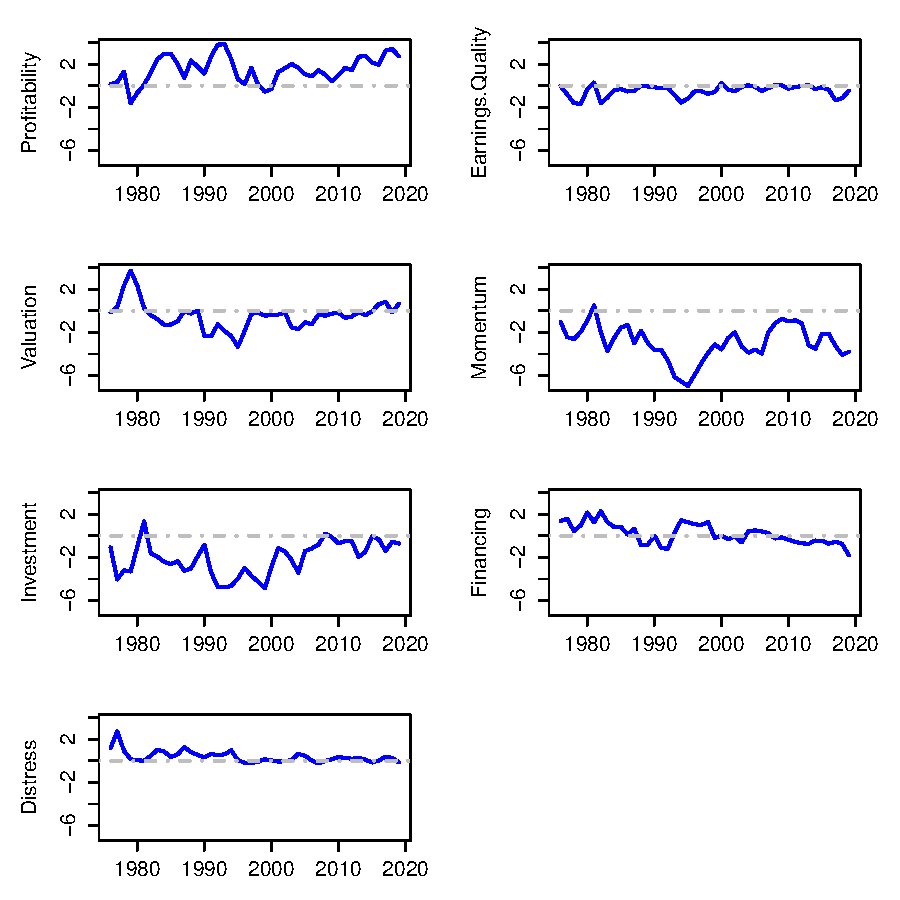
\includegraphics{dropping_one_anomaly_group.pdf}
\end{center}
\end{figure}

\hypertarget{turnover-and-anomaly-deciles}{%
\section{Turnover and Anomaly
Deciles}\label{turnover-and-anomaly-deciles}}

Average turnover ranks for each anomaly decile are presented in figures
\ref{fig:trading_with_anomaly_deciles_1} and
\ref{fig:trading_with_anomaly_deciles_2}.

\newgeometry{margin=1in}
\begin{landscape}
\begin{figure}
\caption{Turnover Ranks and Anomaly Deciles (Part-A)}
\label{fig:trading_with_anomaly_deciles_1}
\subcaption*{Portfolio deciles (x-axis) are constructed each month with respect to each anomaly and average turnover ranks (y-axis) are plotted.}
\rule[0.25ex]{\linewidth}{1pt}
\begin{center}
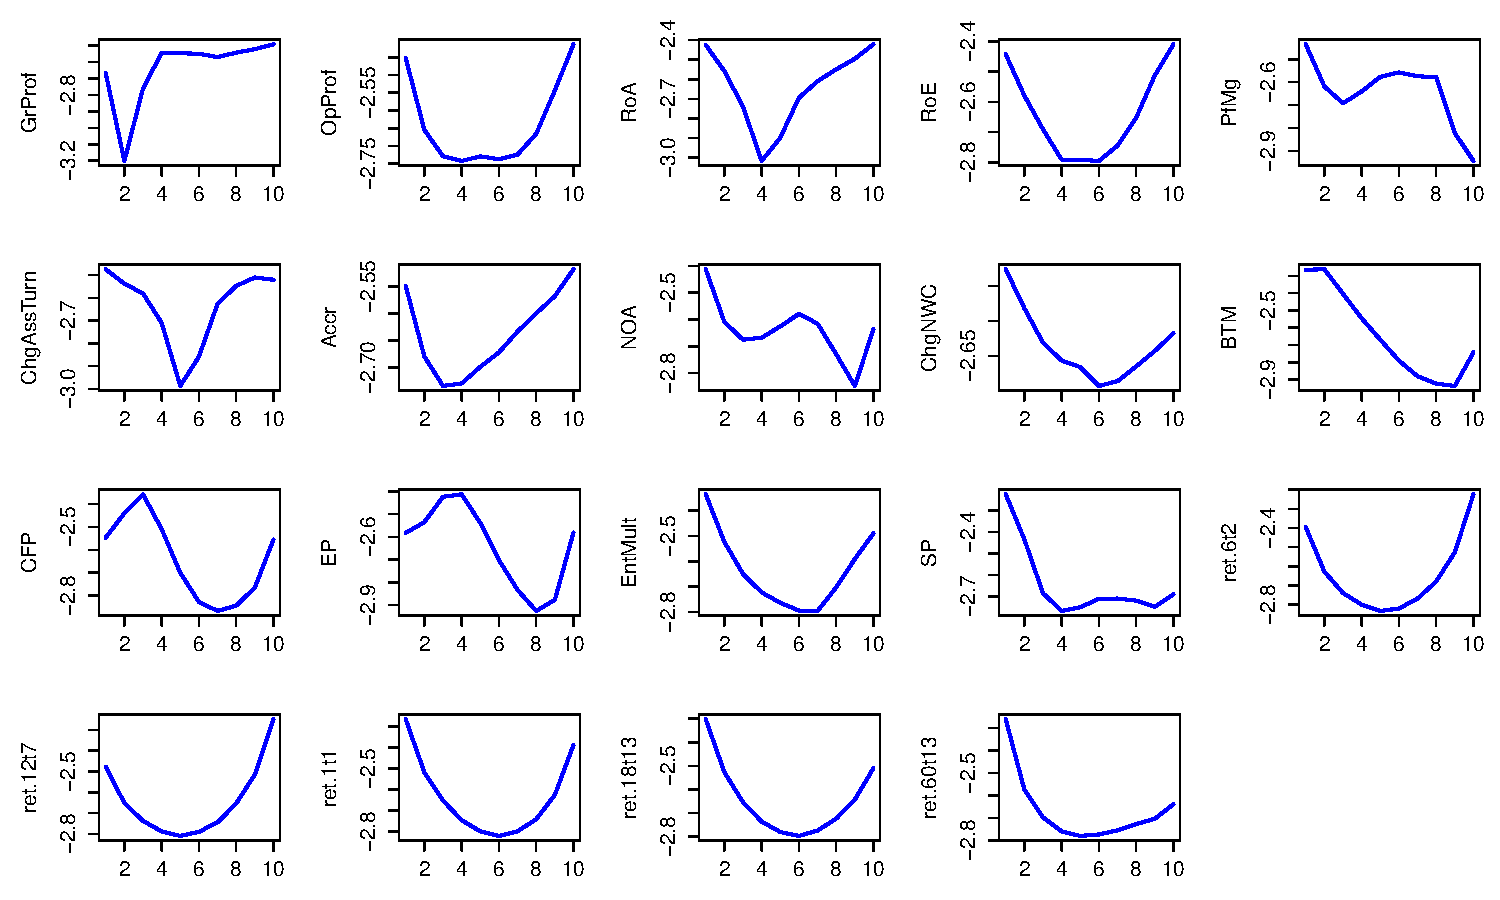
\includegraphics{trading_with_anomaly_deciles_1.pdf}
\end{center}
\end{figure}
\end{landscape}
\restoregeometry

\newgeometry{margin=1in}
\begin{landscape}
\begin{figure}
\caption{Turnover Ranks and Anomaly Deciles (Part-B)}
\label{fig:trading_with_anomaly_deciles_2}
\subcaption*{Portfolio deciles (x-axis) are constructed each month with respect to each anomaly and average turnover ranks (y-axis) are plotted.}
\rule[0.25ex]{\linewidth}{1pt}
\begin{center}
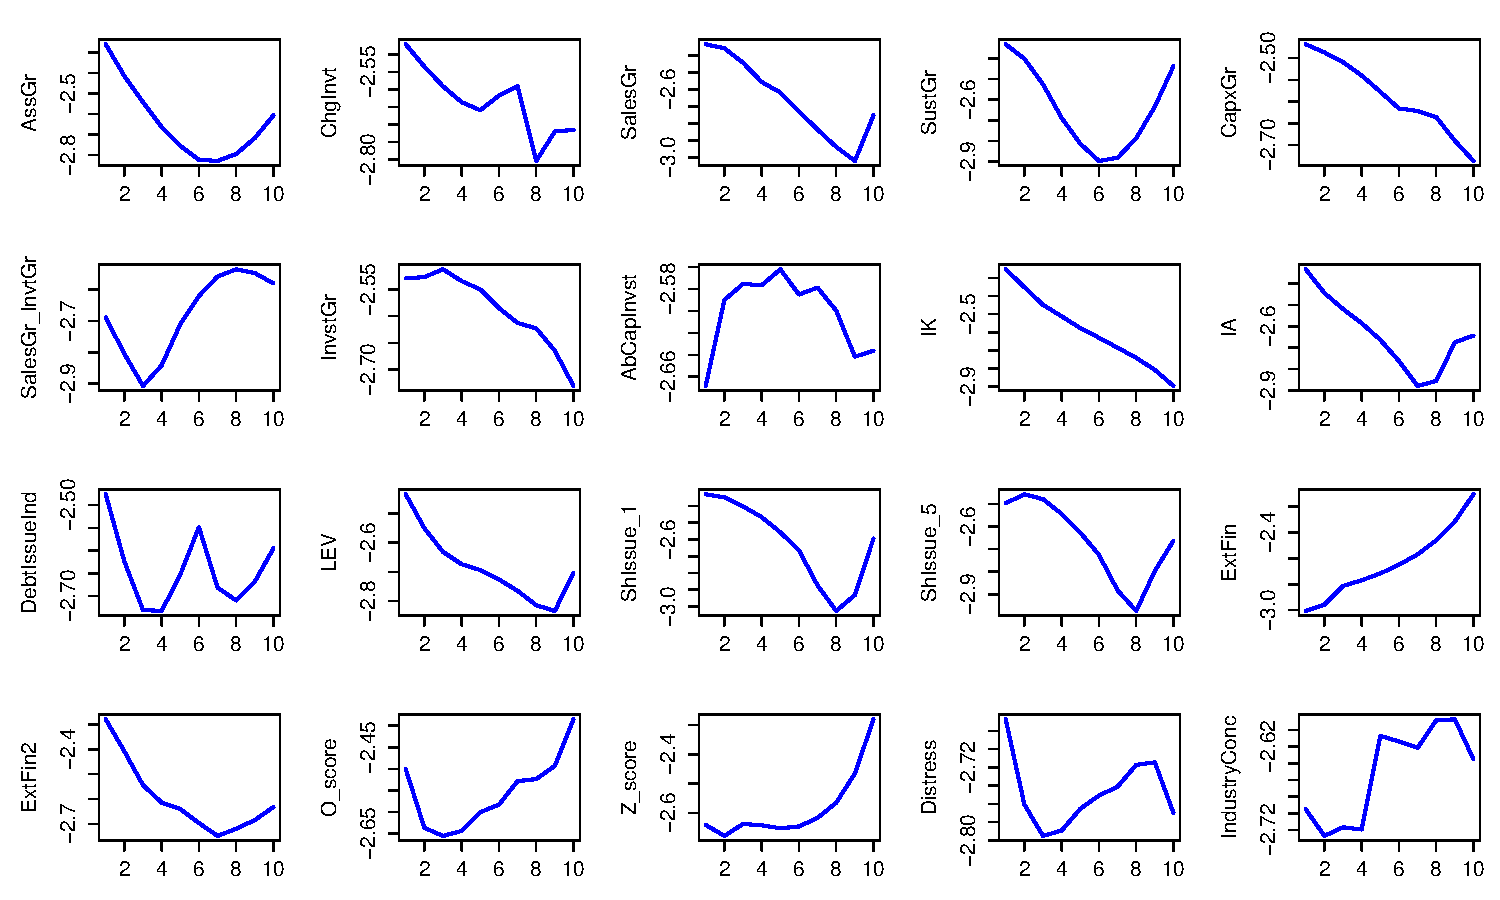
\includegraphics{trading_with_anomaly_deciles_2.pdf}
\end{center}
\end{figure}
\end{landscape}
\restoregeometry

\clearpage

\hypertarget{references}{%
\section*{References}\label{references}}
\addcontentsline{toc}{section}{References}

\bibliography{../bibliography}
\clearpage



\end{document}
